%%%%%%%%%%%%%%%%%%%%%%% file typeinst.tex %%%%%%%%%%%%%%%%%%%%%%%%%%%%%%
%
% This is the LaTeX source for the instructions to authors using
% the LaTeX document class SVMultln with class option 'lnicst'
% for contributions to the Lecture Notes of the Institute for
% Computer Sciences, Social-Informatics and
% Telecommunications Engineering series.
% www.springer.com/series/XXXX       Springer Heidelberg 2007/08/05
%
% It may be used as a template for your own input - copy it
% to a new file with a new name and use it as the basis for
% your article. It contains a few tweaked sections to demonstrate
% features of the package, though.
%
% If you have not much experiences with Springer LaTeX support,
% you should better use the special demonstration file "lnicst.tex"
% included in the LaTeX package for LNICST as template.
%
%%%%%%%%%%%%%%%%%%%%%%%%%%%%%%%%%%%%%%%%%%%%%%%%%%%%%%%%%%%%%%%%%%%%%%%%

%\documentclass[lnicst,sechang,a4paper]{svmultln}
\documentclass{llncs} %this is for NSS
\bibliographystyle{splncs}
%\documentclass[runningheads,a4paper]{llncs} 



\usepackage{amssymb}
\setcounter{tocdepth}{3}
\usepackage{graphicx}


%\usepackage{amssymb}
%\setcounter{tocdepth}{3}
%\usepackage{graphicx}
%\usepackage{fancyhdr}
%\usepackage{lastpage}

\usepackage{url}

%\urldef{\mailsa}\path|{alfred.hofmann, ursula.barth, ingrid.haas, frank.holzwarth,|
%\urldef{\mailsb}\path|anna.kramer, leonie.kunz, christine.reiss, nicole.sator,|
%\urldef{\mailsc}\path|erika.siebert-cole, peter.strasser, lncs}@springer.com|    
%\newcommand{\keywords}[1]{\par\addvspace\baselineskip
%\noindent\keywordname\enspace\ignorespaces#1}


%added by the author himself
\usepackage{subfig}

\usepackage{color}
%\usepackage[numbers]{natbib}
\usepackage{calc}
\usepackage{siunitx}
\DeclareSIUnit\mt{\milli\tesla} %% A method for say short cut or new unit!
\sisetup{inter-unit-product = {-}}

\newcolumntype{P}[1]{>{\centering\arraybackslash}p{#1}}

\usepackage[T1]{fontenc}
\usepackage[ansinew]{inputenc}
\usepackage[english]{babel}
\usepackage{adjustbox}
\usepackage{amsmath,amsfonts,amssymb}
\usepackage{xparse}
\usepackage[section]{placeins} 
\usepackage[misc]{ifsym}
\usepackage{url}

 
\usepackage[many]{tcolorbox}
\usetikzlibrary{decorations.pathreplacing}

%added by kimmo
%\setlength\parskip{12pt}
%\setlength\parindent{0pt}
%\pagestyle{fancy}
%\fancyhf{} 
%\fancyfoot[C]{\thepage\ / \pageref{LastPage}}
%\renewcommand{\headrulewidth}{0pt}



\begin{document}



\mainmatter  % start of an individual contribution

% first the title is needed
\title{Defeating IMSI-Catchers Using Pseudonyms: A DDoS Attack and Solution}
%Concealing IMSI in 5G Network Using Identity Based Cryptography

% a short form should be given in case it is too long for the running head
%\titlerunning{Concealing IMSI Using Identity Based Encryption} 


% the name(s) of the author(s) follow(s) next
%
% NB: Chinese authors should write their first names(s) in front of
% their surnames. This ensures that the names appear correctly inlso
% the running heads and the author index.
%
\author{Mohsin Khan$^\text{1(\Letter)}$%
%%\thanks{Please note that the LNICST Editorial assumes that all authors have used
%%the western naming convention, with given names preceding surnames. This determines
%%the structure of the names in the running heads and the author index.}%
\and Kimmo J\"arvinen$^\text{1}$
\and Philip Ginzboorg$^\text{2}$
\and Valtteri Niemi$^\text{1}$
}  %

%\authorrunning{Mohsin Khan \and Valtteri Niemi}

% (feature abused for this document to repeat the title also on left hand pages)

% the affiliations are given next
\institute{$^\text{1}$University of Helsinki, Helsinki, Finland\\
\{\email{mohsin.khan, kimmo.u.jarvinen, valtteri.niemi}\}\email{@helsinki.fi}\\
$^\text{2}$ Huawei Technolgies\\
\email{philip.ginzboorg@huawei.com}
%P.O. Box 68 (Gustaf H\"allstr\"omin katu 2b)\\
%FI-00014 University of Helsinki\\
%Finland\\
%\url{https://www.cs.helsinki.fi/en}
}

%relationship stu
%
% NB: a more complex sample for affiliations and the mapping to the
% corresponding authors can be found in the file "lnicst.dem",
% that is contained in the LNICST LaTeX support package.
%

%%%\toctitle{Lecture Notes in Computer Science}
%%%\tocauthor{Authors' Instructions}
\maketitle


\begin{abstract}
IMSI-catchers are still in existence in all the 3GPP defined cellular networks. Pseudonym based solutions to defeat IMSI-catchers have been published in the recent years. We have found one vulnerability in these solutions. The vulnerability enables an attacker to convince the home network (HN) to forget an old pseudonym of a legitimate UE and compute a new one. The attacker does not need any participation of the legitimate UE to mount this attack. A malicious UE or a serving network (SN) can exploit this vulnerability to kick a legitimate UE out of service. We show that, exploiting this vulnerability, a novel DDoS attack can be mounted against an entire cellular network. The attack can send 50 percent of the UEs out of service using a reasonably large botnet of mobile users. We justify our claim by an analytical argument backed by a simulation. Even though, in principle, a malicious SN can also exploit the vulnerability, we argue that the SN can not gain anything meaningful before the attack is detected and stopped. Besides, an SN can behave maliciously in other even more fatal ways. Hence it is not important to protect against a malicious serving network in this context. We present a solution to fight against the DDoS attack by piggybacking the location update message sent by the serving network to the home network. We present a qualitative analysis of our solution. We argue that our solution is immune to the the DDoS attack and still protects the identity privacy, and remains backward compatible with the legacy networks. We also discuss other practical issues of the usability of pseudonyms from charging and lawful interception point of view that appear to be ignored so far.
\keywords{3GPP $\cdot$ IMSI-catchers $\cdot$ Pseudonym $\cdot$ Idenity $\cdot$ Privacy}
\end{abstract}


\section{Introduction} \label{intro}
International mobile subscriber identity (IMSI) is the global identifier of a mobile phone subscriber. IMSI-catchers are devices that can create a list of IMSIs of the subscribers present in a certain geographical area. IMSI catching is an identity privacy problem. The problem has been known for long but still prevailing in all the 3GPP defined cellular networks (GSM, UMTS, LTE) for decades \textcolor{red}{cite}. 

\subsubsection{How IMSI-catchers catch IMSI?} A subscriber's user equipment (UE) has to identify itself to the network before connecting. The identification message has to be sent in plain-text because the security of the network is based on symmetric key cryptography \textcolor{red}{cite}. In symmetric key cryptography, a secret key has to be shared before starting any encryption. The home network (HN) stores a secret key for every subscriber in the subscriber database. The secret keys are also securely stored in the respective subscriber identity module (SIM). However, the HN needs to know the identity of the subscriber to choose the right secret key to start encrypting or decrypting any message. So, when an unknown UE appears, the network makes an IMSI inquiry to the UE . Consequently, the UE has to sent the IMSI in plain-text \textcolor{red}{cite}. 

A passive IMSI-catcher who is just listening to the radio channel can read the identification message. An active IMSI-catcher who sets up a fake base station and impersonates a legitimate serving network (SN), do an IMSI inquiry to all the UEs that try to connect. The UEs respond with their respective IMSIs in plain-text \textcolor{red}{cite}. See Figure \ref{fig:IMSI-catching}. 

\begin{figure}[!tbp]
  \centering
  \begin{minipage}[b]{0.44\textwidth}
    \includegraphics[width=\textwidth]{Passive_IMSI-Catcher.eps}
%    \caption{Legitimate SN}
  \end{minipage}
  \hfill
  \begin{minipage}[b]{0.50\textwidth}
    \includegraphics[width=\textwidth]{Active-IMSI-Cactcher.eps}
%    \caption{IMSI-catcher}
  \end{minipage}
  \caption{IMSI-catcher}
  \label{fig:IMSI-catching}
\end{figure}

\subsubsection{What an IMSI catcher can do with the caught IMSIs?} With the caught IMSIs, an IMSI catcher can monitor who are coming and leaving a certain geographical area \textcolor{red}{cite}. An IMSI catcher can also track the locations of a targeted individual \textcolor{red}{cite}. There are other range of more sophisticated active man in the middle attacks that start with catching the IMSI of a subscriber, e.g., attacking the confidentiality of user data by downgrading the air interface encryption \textcolor{red}{cite}. Now a days, all these advanced attackers are called IMSI-catchers. However, in this paper, we will limit our discussion to the attackers who only gathers a list of IMSIs.

\subsubsection{How available IMSI-catchers are in real life?}

\subsubsection{Current state of art in defeating IMSI-catchers}

\subsubsection{Our Contribution}

\subsubsection{Overview}


\section{Background}

\subsubsection{Identification in the existing networks}
\subsubsection{Authentication in the existing networks} we need to discuss the authentication mechanism because the pseudonym based approach uses the messages in the authentication protocol to piggyback the messages required to be sent across.
\subsubsection{How pseudonym based solution works}


\section{Vulnerability of Pseudonym Based Solutions}
The fundamental idea of all the pseudonym based solutions \cite{CCS15,SSR15,Ginzboorg_Niemi_2016,Norrman_Naslund_Dubrova_2016} are essentially same. When a certain old pseudonym is  used by a user, the HN computes a new pseudonym, associate the new pseudonym to the respective IMSI and forget a certain old pseudonym. Forgetting an old pseudonym is important so that it can be reused. 

When a fake UE (FUE) uses a random pseudonym and if by chance, the random pseudonym is associated with a legitimate UE, the network forgets an old pseudonym for the legitimate UE. The network also computes a new pseudonym which the legitimate UE has no knowledge of. If the network remembers  $k$ number of used pseudonyms before forgetting any, the FUE needs to make the attack $k+1$ times so that the network forgets all the pseudonyms that the legitimate user possesses. This is a fatal damage to the identity of the UE, because all the successive authentications of the UE will fail. If there are $n$ number of subscribers in an HN, then the probability of the above attack being successful is $\frac{n}{10^{10(k+1)}}$, which is apparently a tiny probability. However, in Section \ref{section:DDoS}, we will show how this tiny probability can be exploited into a fatal DDoS attack. We will use the BVR scheme to demonstrate the attack, \textcolor{red}{eve though similar attacks can be mounted against the other schemes also.}


\subsection{The DOS Attack Against the BVR Scheme}
In the BVR scheme, a subscriber $s$ has two pseudonyms $\left(s_p,s_p'\right)$ in the HN and two pseudonyms $\left(PMSI,P_{new}\right)$ in the UE. In an ideal case, $PMSI = s_p, P_{new} = s_{p'}$. 

The attack is mounted by an FUE. The FUE sends a random pseudonym $q_1$ to a legitimate SN. The legitimate SN forwards the pseudonym to the respective HN. If by chance, $q_1 = s_{p'}$, the HN forgets $s_p$ and sets $s_p \leftarrow s_{p'}$. The HN also generates an unused pseudonym ${p''}$ and sets $s_{p'} \leftarrow p^{''}$. As a result, in the HN, the current  pseudonym-state for the subscriber $s$ is $\left(s_{p} = P_{new},s_{p'} \neq PMSI,P_{new}\right)$. At this stage, there is only one pseudonym present both at the UE and HN.

The FUE sends another pseudonym $q_2$ and if again by chance, $q_2 = s_{p'}$, then the HN again forgets $s_{p}$, sets $s_p \leftarrow s_p'$. HN also generates an unused pseudonym $p'''$ and sets $s_{p'} \leftarrow p'''$. Consequently, in HN, the current pseudonym-state of subscriber $s$ becomes $\left(s_{p} \neq PMSI,P_{new},s_{p'} \neq PMSI,P_{new}\right)$. If there were no pseudonyms exchanged in between the HN and the legitimate UE while the attack was mounted, the pseudonym-state of the UE remains as $\left(PMSI,P_new\right)$. So at this state there is no pseudonym present at both of the UE and HN sides. See Figure \ref{fig:dos_attack}. The next time the user would need to authenticate itself to a network, the authentication will fail and hence be denied any service.

\begin{figure}[]
  \centering
    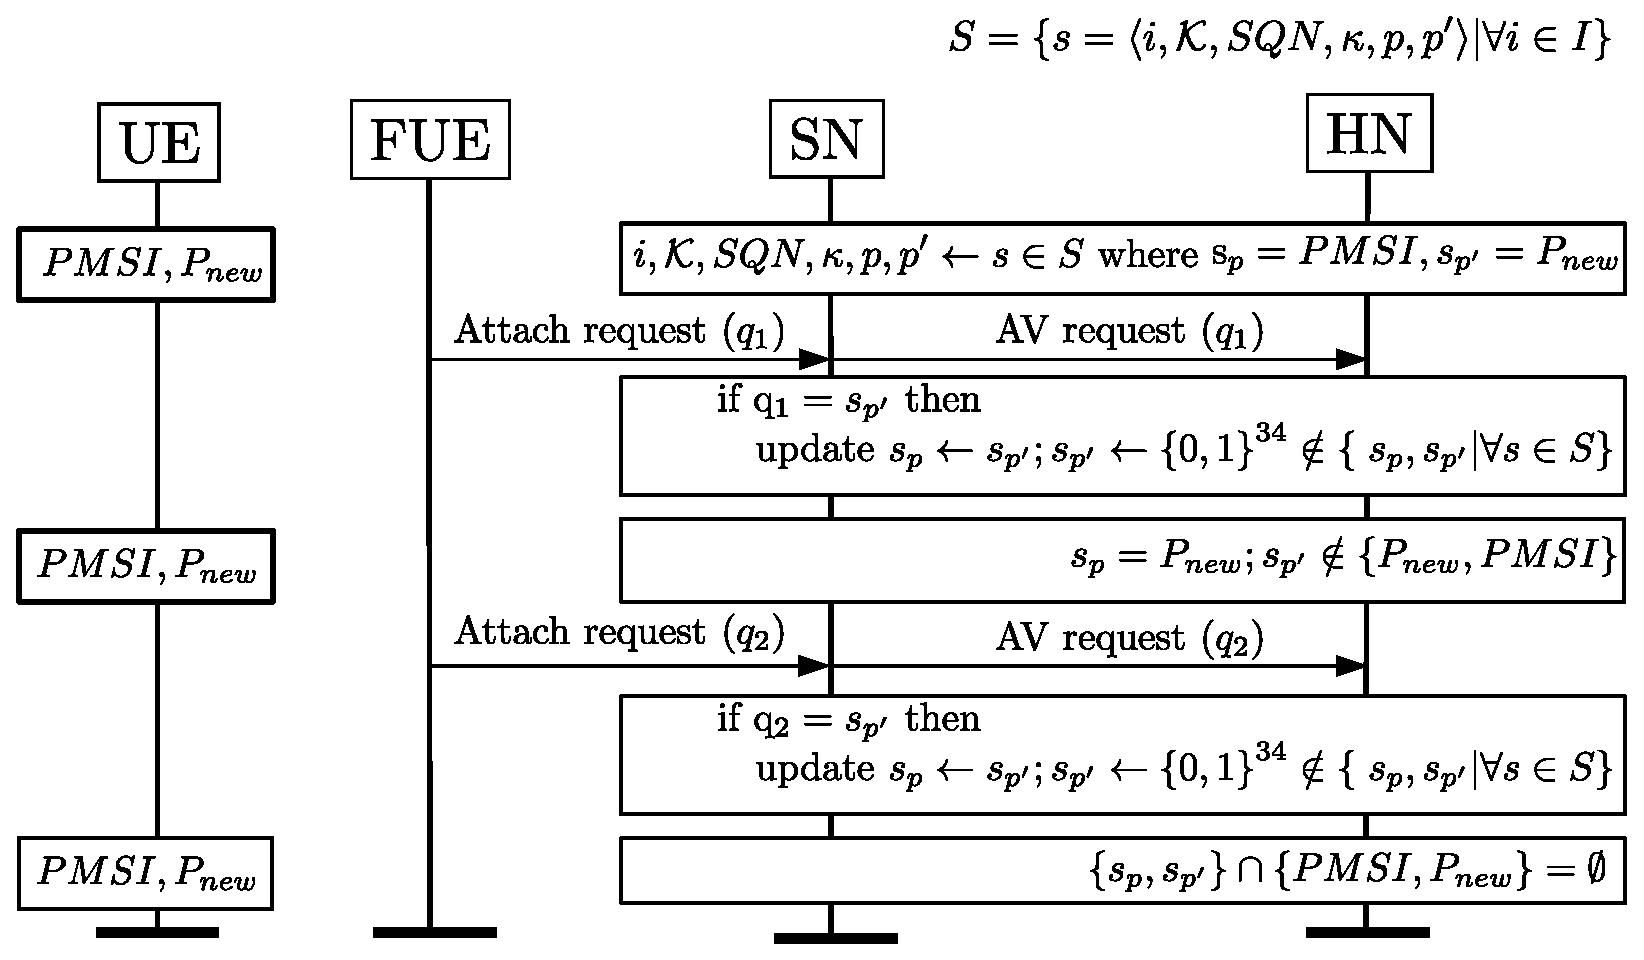
\includegraphics[width=\textwidth]{DDoS.eps}
  \caption{A DoS Attack against the BVR scheme}
  \label{fig:dos_attack}	
\end{figure}

If the probability of success of the above attack to a targeted user is $\frac{1}{10^{20}}$. The probability of   success of the attack to any user is $\frac{n}{10^{20}}$. This is a tiny probability. But in Section \ref{sec:DDoS}, we show that a very efficient and fatal DDoS attack can be mounted using by exploiting this tiny probability.

\subsection{The DDOS Attack}
In the DDoS attack, many FUEs send many pseudonyms to the targeted HN via a legitimate SN. The HN processes the pseudonyms as they arrive. Let us assume, the total number of pseudonyms sent to the HN is a large integer $m$. In this case, a user $s$ will be affected by the attack if there exists two integers $0 < x < y \leq m$ such that $q_{x} = s_{p'}$ and $q_{y} = s_{p'}$. We have considered two different ways to mount this attack. In one way, the pseudonyms that are sent to the network are chosen randomly with replacement, which means the attack might sent one pseudonym more than once to the network. In the other way, the pseudonyms are chosen without replacement, which means the attack send one pseudonym only once.

\subsubsection{With replacement}
In this case, the expected number of affected users $E[u_a]$ is
\begin{eqnarray}
E\big[ u_a \big] &=& n\left(1- \left(1 - \frac{1}{10^{10}}\right)^m - m\left(\frac{1}{10^{10}}\right)\left(1 - \frac{1}{10^{10}}\right)^{\left(m-1 \right)} \right)
\end{eqnarray} 

See Appendix \ref{appendix: A} for the derivation. We have run a simulation of this attack and found that above model is fairly accurate. See Figure \ref{fig:simulation_and_modeling}.

\begin{figure}[]
  \centering
    
\includegraphics[width=\textwidth]{sim_and_mod.pdf}
  \caption{Success Rate of the DDoS Attack. IMSI space $10^{10}$. Number of subscribers in HN is $10^7$. The black and blue line presents the expected number of affected users in case of the with and without replacement attacks respectively. Under the black line, there are three red lines which represent the results of three simulations of with-replacement attack. Under the blue line, there are three green lines which represent the results of three simulations of without-replacement attack.}
  \label{fig:simulation_and_modeling}	
\end{figure}

\subsubsection{Without replacement}
In this case the attacker runs two rounds of the attack. In the first round the attacker sends all the pseudonyms in the IMSI-space without replacement, means each pseudonym is sent exactly once. Once the first round is completed, the attacker runs the attack for one more round. However, after sending $m$ number of pseudonyms to the network, the expected number of affected users $E[u_a]$ is
\begin{eqnarray}
E\big[ u_a \big] = \begin{cases} \frac{m^2}{2\cdot 10^{10}}, & \mbox{if } 0 < m \leq 10^{10} \\ 
2m - 10^{10} - \frac{m^2}{2\cdot 10^{10}}, & \mbox{if } 10^{10} < m \leq 2\cdot 10^{10} \end{cases}
\end{eqnarray} 
See Appendix \ref{appendix: A} for the derivation. We have run a simulation of this attack and found that above model is fairly accurate. See Figure \ref{fig:simulation_and_modeling}. Note that, this is an estimation where the without-replacement attack is not a distributed attack. Rather the attack is mounted by only a single FUE. In case of distributed without-replacement attack, the expected number of affected users will be less than what is shown in the plot. However, we believe that, the distributed without-replacement attack will have higher number of affected users than that of distributed with-replacement attack.



\subsection{Why SN is not a Potential Adversary}


\subsubsection{Modeling and Simulation}


\section{Solution}

\section{Analysis}
\subsubsection{why the solution is good}
what happens in the error cases

\section{Related work}
how good the newest paper really is

\section{Usability of pseudonyms}



\section{Conclusion}
\label{sec:conclusion}


\subsubsection{Acknowledgement.}
\label{sec:acknowledgement}


\bibliographystyle{splncs}
\bibliography{ref}{}

\begin{thebibliography}{5}



\end{thebibliography}

\end{document}
